\chapter*{APPLE, EL PADRE DE LA REVOLUCIÓN DE LOS SISTEMAS OPERATIVOS MÓVILES}

En este capítulo damos a conocer porque la compañía APPLE
está tan destacada con su nueva
implementación de IOS, como un novedoso
sistema operativo para celulares, sus grandes
desarrollos, pasos e incluso su gran estabilidad
económica, lo cual hace interesante este
capítulo. También las nuevas tecnologías y por
supuesto de donde surgieron, quien las
implementó y cómo fue su histórico desarrollo.
Nos basamos, en que sabemos que APPLE no
inventó; pero sí creo la revolución de los
ordenadores, reproductores mp3, celulares,
Tablets gracias a su diseño novedoso y la gran
garantía de seguridad tanto software como
hardware. Indiscutiblemente Apple ha sido de
gran influencia para nuestra sociedad.

Aunque Apple no inventó la telefonía móvil, si es cierto que ha
reinventado el paradigma actual de estos, y ha marcado el
camino para sus competidores. iOS es el sistema operativo que
utilizan los iPhone, iPad y ipod. Su principal base es ofrecer una
experiencia única al usuario.

Por otro lado los desarrolladores de IOS, también se preocupan
por garantizar que cualquier persona pueda acceder a sus
aplicaciones y especialmente a cualquier dispositivo con IOS, lo
cual ha demostrado no solo su desarrollo tecnológico sino
también su gran labor social. Esto hace referencia a su nuevos
desarrollos de software, que son enfocados exclusivamente para
personas con dificultades de visión, audición, Lectura, escritura,
aprendizaje, físicas y motoras.

\section*{STEVE JOBS, UNA MENTE BRILLANTE}

Apple desde sus comienzos ha sido una de las empresas que ha
revolucionado el mundo con sus invenciones en lo que
dispositivos electrónicos respecta, muestra de ello fue crear la
primera fábrica automatizada de computadores, la primera
computadora personal, pionero en el uso de iconos y ratón para
controlar un computador eso era lo más innovador del momento
a todo el mundo le encanto esta tecnología por y fue así como
Apple tuvo su primer éxito Steve Jobs y Steve Wozniak sus
creadores tenían tan solo 21 y 26 años cuando lanzaron su
primera computadora, la Apple1 y tuvo tanto éxito al cabo de 5
años la empresa había recaudado cientos de millones de dólares,
luego de esto a la empresa se disparó como un cohete en mayor
parte gracias al ingenio y la creatividad de Steve Jobs.

\section*{INICIOS DEL IPHONE}

El iPhone no era el primer teléfono con pantalla táctil pero si
era el primero en responder con precisión y fluidez tampoco el
primero con internet pero si era el primero que lo hacía cómodo
y ágil, tampoco era el primer teléfono que incluía fotos video,
música o juegos aunque revolucionó sus posibilidades la
segunda versión del iPhone trajo consigo las muy cotizadas las
tecnologías 3g y GPS también trajo la segunda versión del ios
este incluía App store la tienda que generó miles de empleos de
trabajo y miles de millones de dólares de beneficio por vender
aplicaciones baratas al momento de sacar el iPhone 3g android
cogía fuerza.
Los ingenieros de Apple investigaron la mejor manera para
crear el que sería el dispositivo insignia de la marca. Para ello
tenía en mente varias tecnologías novedosas para el momento
una de ellas fue el gorilla glass que consiste en una pantalla muy
resistente a golpes y rallones, pero esta tecnología podría
aumentar los costos de producción del iphone ya que este cristal
era muy caro de producir y hasta el momento no existía una
empresa que fuera capaz de producir este cristal a gran escala
otra tecnología era un avanzado sistema operativo que fuera de
la más la calidad Apple, además de esto el presidente de Apple
Steve Jobs era un sujeto obsesionado con la presentación de su
producto ya que para él la tecnología no solo tenía que ser
funcional sino también tenía que ser bello y agradable al
usuario, hasta el más mínimo detalle gráfico tenia era
meticulosamente revisado para que este fuera el más llamativo
sistema operativo del momento.

Toda la tecnología que implementó Apple en su celular tuvo un
costo de 150 millones de dólares en investigaciones y diseño.

Bill Gates opinó al respecto sobre el iPhone dijo que este celular
no iba a tener éxito ya que era muy caro y superaba por mucho
el precio cualquier dispositivo en el mercado hasta el momento.
Para sorpresa de todos, Apple vendió 270 mil iPhones en las 30
primeras horas después de su lanzamiento y en el 2007 8
millones de iPhones se vendieron en Estados Unidos EEUU
según la Entertainment Software Association. Luego de su éxito
Apple lanzó varias versiones pero cada una de ellas ha tenido la
particularidad de que todas sus configuraciones (botones) en el
sistema operativo han estado en el mismo lugar con el fin de no
confundir al usuario “cosa que no pasa con android”. Sin
embargo muchos han desertado del iPhone ya que su sistema
operativo cerrado no le permite al usuario hacer modificaciones
a su antojo y únicamente se puede interactuar a través de la
aplicación ITunes “reproductor multimedia de Apple”,
continúa…

Apple vendió un millón de iPhone 3G en sus 3 primeros días de
venta.

\section*{BREVE HISTORIA DE IOS}
en un comienzo iOS fue lanzado en enero del 2007 con el
nombre de iPhone OS puesto que aún se usaba únicamente en el
iPhone, luego septiembre del mismo año fue implementado en
el ipod touch pero solo fue hasta el 2010 que el sistema
operativo pasaría a ser llamado iOS durante el lanzamiento del
iPhone 4 en septiembre de 2013 fue lanzado iOS 6 durante la
presentación del iPhone 5 en junio del siguiente año fue
presentado iOS 7, este último fue el mayor cambio de iOS desde
el iPhone original, Cambia por completo el diseño gráfico del
sistema, haciéndolo más plano con nuevos iconos, trae nuevas
características como AirDrop, filtros de cámara, fondo dinámico
entre muchas otras, ese mismo día en la misma conferencia de
dieron datos oficiales fueron conocidos de que hasta la fecha se
han vendido más de 600 millones de iDevices, los usuarios de
iOS utilizan un 50\% más sus dispositivos que los de Android, el
mercado web lo domina iOS con un 60\% y en tabletas el iPad
tiene el 82\% del tráfico web, se ubica en el lugar #1 de
satisfacción al cliente con un 73\% seguido por Windows Phone
con el 53\%, y el 93\% de los usuarios tienen instalada la versión
actual del sistema.

\section*{PRINCIPALES CARACTERÍSTICAS DE IOS}
\subsection*{PANTALLA PRINCIPAL}

La pantalla principal (“llamada SpringBoard”), es donde se
ubican los iconos de las aplicaciones y en la parte inferior
donde se pueden anclar aplicaciones de uso frecuente, aparece
al desbloquear el dispositivo o presionar el botón de inicio. La
pantalla tiene una barra de estado en la parte superior para
mostrar datos, tales como la hora, el nivel de batería, y la
intensidad de la señal. El resto de la pantalla está dedicado a la
aplicación actual.

\subsection*{CARPETAS}

posible acceder a las carpetas del sistema operativo, la única
manera de acceder a ellas es a través de el jailbreak, que
mencionaremos más adelante, Apple insiste en cuidar la
integridad de su sistema operativo. Para ello ha creado una
interfaz que unicamente permite al usuario ver iconos de las
aplicaciones instaladas, y a través de ellas se accede a la
información de todo el dispositivo. no existe un escritorio, como
el que se ve en android, en vez de ello muestra todos los iconos
de aplicaciones en un menú dinámico y atractivo.
IOS tiene un sistema simple de carpetas. Se puede mover una
aplicación sobre otra y se creará una carpeta, y así se pueden
agregar más aplicaciones a esta mediante el mismo
procedimiento. Pueden entrar hasta 12 y 20 aplicaciones en el
iPhone y iPad respectivamente. El título de la carpeta es
seleccionado automáticamente por el tipo de aplicaciones dentro
de ella, pero puede ser editado por el usuario.

\subsection*{SEGURIDAD}

Los virus y el malware ya no son solo problema de los
ordenadores de mesa, también pueden atacar a dispositivos
móviles. Apple se preocupa por la seguridad de iOS.

Apple tenía la mirada puesta para crear uno de los mejor
sistemas operativos. Para ello dedicó mucho tiempo a su diseño
y seguridad. en el desarrollo de IOS se pensó en la mejor
manera de proteger la integridad de su núcleo y de los archivos
de su sistema operativo, lo que llevó a los ingenieros a crear
múltiples restricciones a los usuario, tales como: acceso
restringido a limitado o nulo a las carpetas de IOS, únicamente
se pueden instalar aplicaciones aprobadas y autorizada por
Apple y en lo esencial que el usuario no intervenga en los
procesos que mueven el sistema operativo. Al final Apple logró
crear uno de los sistemas operativos más estables, pero con un
costo alto de personalización y control del dispositivo.

El software está diseñado para defenderse de malware y virus,
en ademas sabemos que iOS se ocupa de proteger la
información personal. Y para garantizar aún más la seguridad,
también es posible poner una contraseña que impida el acceso
no autorizado a tu dispositivo. Al usarla, iOS cifra tu correo
electrónico y todas las apps de terceros para protegerlos.


\subsection*{MULTITAREA}

La multitarea llega en la generacion de IOS 4, la cual permite
poder abrir varias aplicaciones a la vez, esto quiere decir poder
ejecutar varios procesos, sin que se sature el procesador, es una
característica en las nuevas tecnologías. Por lo cual optimizan
los rendimientos de la máquina y permite por ejemplo que la
batería dure aún más tiempo.

IOS permite pasar de una app a otra de manera rápida,
mientras una aplicación está funcionando durante un breve
periodo de tiempo e ir luego a estado de suspensión. IOS
tiene un óptimo control del sistema en el momento que el
dispositivo se active nuevamente.

Muchas aplicaciones pueden estar abiertas en segundo
plano. Para aumentar el rendimiento del procesador y de la
batería IOS pondrá en suspensión la aplicación que está en
segundo plano en el momento que lo considere más
adecuado, como por ejemplo cuando la red Wi-Fi no la está
utilizando ninguna aplicación.

\subsection*{KIT DE DESARROLLO}

En 2008 Apple lanzó el kit de desarrollo o SDK permitiendo que
desarrolladores externos que quieran desarrollar sus
aplicaciones para iOS.

De cualquier manera, solo es posible utilizar el app en los
dispositivos después de pagar una cuota de 9,99 dolares por mes
al iPhone Developer Program. (Comunidad de desarrolladores
iOS).

Los desarrolladores pueden distribuir sus aplicaciones a través
de la App Store y ponerle precio por encima de 0,99 dólares,
donde recibirán el 70\% del dinero recaudado por las creaciones.
El desarrollador puede optar por lanzar la aplicación gratuita, y
de esta forma no pagar ningún costo por distribuir la aplicación.
(excepto por la cuota de la membresía).

\subsection*{ECONOMÍA IOS}

Apple como cualquier otra compañía se dedica a actividades
con fines económicos o comerciales, por lo tanto ha tenido unos
buenos resultado y una estabilidad económica en el tiempo. lo
impresionante son los cambios drásticos que tuvo la compañía,
cuando surgió la revolución del sistema operativo de las nuevas
tecnologías, las cuales permitieron unas grande ganancias y
desarrollo.

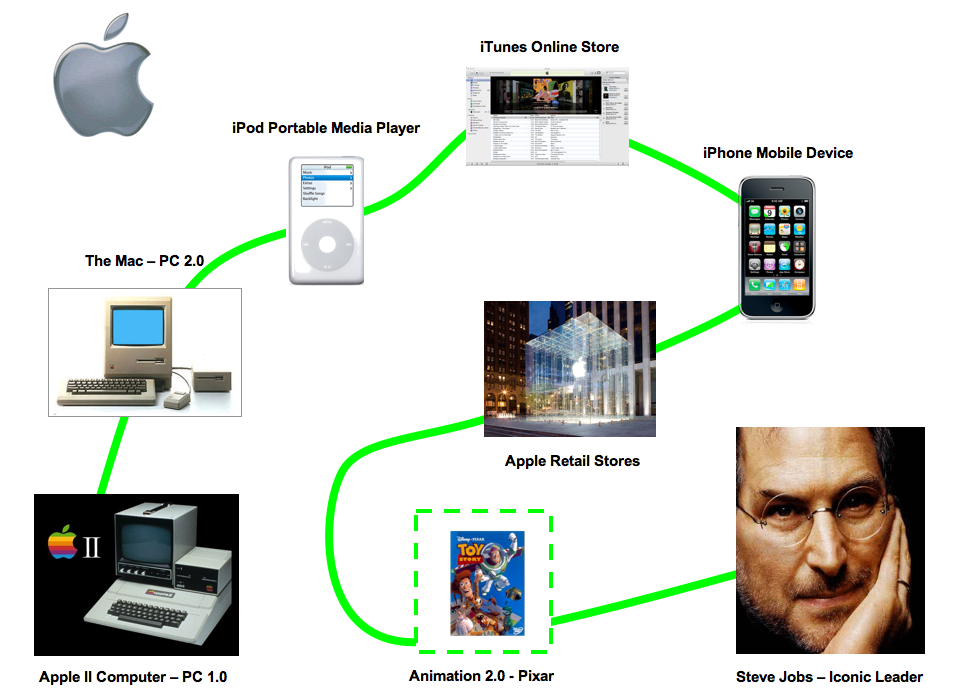
\includegraphics[scale=0.5]{img/cp08/img0801.png}

Según esta gráfica podemos afirmar que su grandes ganancias
económicas fueron a inicios del 2001, pero vemos que a partir
del 2010, cuando fue lanzado el IOS 4 hasta la muerte de Jobs
superan todas las ganancias de la historia de APPLE. Esto nos
confirma que IOS es un sistema operativo verdaderamente
revolucionario en la tecnología.

Después de la muerte de Steve Jobs, gran parte de la
comunidad pensó que iba hacer un gran golpe
para la marca de la manzana, aunque si
hubieron cambios tanto en el interior, como el
panorama exterior. pero eso no fue impedimento
para que esta empresa siguiera con sus grandes
éxitos economicos.

Estas fueron las principales transformaciones por la que ha
pasado Apple desde la muerte de Steve Jobs
llevó a la marca a manos de Tim Cook:

1. Google es ahora el principal competidor de Apple:
Samsung sigue siendo el “enemigo” de Apple en el mercado de
smartphones y tabletas, pero Google supone un gran reto para el
nuevo mercado que está abriendo Apple, los sistemas de
almacenamiento en la nube.

2. Apple es ahora un sitio mejor para trabajar: Apple ha
seguido el modelo de lugar de trabajo amable de las otras
compañías punteras, y en vez de presión e intimidación, Apple
apoya a sus trabajadores con incentivos.

3. La tecnología “que se pone” es el futuro: parece que
Apple ya ha encontrado el nuevo hueco en el mercado donde
innovar y revolucionar, el iWatch, o reloj inteligente puede
suponer el inicio de algo grande y el nuevo invento que los fans
llevan tanto tiempo esperando.

4. Apple versus Samsung: Apple consiguió ganar a Samsung
en los juzgados, pero en cifras de ventas y popularidad la cosa
está muy reñida.

5. Apple ya no es una dictadura: las decisiones son tomadas
por un comité y no por Steve Jobs de manera unilateral.

6. ¿Qué pasa con la Apple TV?: con la muerte de Steve Jobs se
paralizaron los planes de la Apple TV, y parece que todavía no se
han retomado, aunque el futuro dirá.

7. La estrategia de marketing ha cambiado: Steve Jobs era
considerado el mejor “marketero” de todos los tiempos. Su
estrategia basada en la simplicidad se ha perdido con su
fallecimiento, centrándose la marca en vender otros aspectos.”

\section*{IMPACTO SOCIAL}

Si se sabe que efectos ha tenido IOS en el sociedad, tenemos
que saber que el IOS permitió la optimización de tres productos;
como primera medida un teléfono móvil, un iPod táctil (que para
ese tiempo era solo un reproductor de música) y aplicaciones
para tener conectividad a internet, en sus primeros pasos en
2001 estas funciones dieron a Apple la ventaja amplia en el
mercado de tecnología móvil.

En 2009 OCU realizó una encuesta a 700 personas
preguntándoles ¿para qué utilizamos el iPhone? Y se encontró
que la mayoría utilizan su teléfono para utilizar sus aplicaciones
de internet, redes sociales y de correo electrónico
Foro iPhone. Encuesta Ocu, ¿para que utilizamos el
iPhone? [electrónico] Recuperado el 21 de Agosto de 2010
de http :// www . actualidadiphone . com / foro / viewtopic . php ?
f =1& t =3616

Antiguamente se utilizaban los libros para buscar información,
hoy día se utilizan las herramientas que brindan los sistemas
operativos móviles como IOS para tener rápidamente la
información que necesite el usuario, incluso se pueden utilizar
las múltiples aplicaciones que posee la Apple Store, que
permiten una amplia gama de funciones como el GPS con mapas
de todo el mundo, es posible encontrar aplicaciones de yoga,
actividades de ejercicio físico, entretenimiento, retos mentales.
Los usuario de IOS descargan hasta nueve aplicaciones por mes,
y estas descargas van desde contenidos musicales, juegos a las
aplicaciones de redes sociales.

De otra parte el impacto de IOS, se ve reflejada en la educación,
IOS brinda la posibilidad de acceder a cursos virtuales a través
de sus aplicaciones que permite tener contacto directo con el
contenido que ofrecen las universidades. Un caso destacado es
el de Monterrey que facilita el beneficio de universidad virtual y
se puede estudiar online de una manera muy práctica, dando así
oportunidades a las personas que buscan alternativas de estudio
más económicas.

En conclusión la opción de estar conectado a internet en todo
momento ya es necesario para todos los sistemas operativos
móviles para el día a día de las personas, ya no es una elección
conformarnos con lo necesario, podemos instalar aplicaciones
multimedia, entretenimiento y muchas otras aplicaciones, ahora
nuestro dispositivo móvil se ha convertido en un compañero
inseparable. Todo esto es posible gracias al innovador sistema
operativo IOS. Ahora es posible llevar la oficina en nuestros
dispositivos móviles, escribir archivos Office, con una gran
rapidez de proceso.

\section*{IMPACTO DE DEPENDENCIA MÓVIL}

El gran desarrollo de tecnología movil a provocado que
numerosas personas tengan problemas de adicción con un
celular, ya que hay personas que están sufriendo cuando olvidan
el movil en su casa, se quedan sin cobertura o sin bateria. Lo
que se convierte en un problema global.

Ahora en esta era de competencia, apple intenta buscar
alternativas para mejorar sus mercados, por lo tanto incorpora
nuevos diseños para los chips para sus dispositivos ios. Esto
ocurre cuando la compañía coreana (Samsung ) inicia a fabricar
los chips a partir de los diseños de apple. esto tiene que ver
mucho con las dependencia de los celulares, porque las
compañías compiten solo porque las personas usen más los
dispositivos móviles que otros y por esos su diseños atractivos.

\section*{COMO EL IOS CAMBIÓ EL MUNDO}

Luego de la muerte de Steve Jobs, hubiese sido fácil enaltecer
su nombre con sus múltiples inventos y enseñanza pero este
genio no era –ni mucho menos- un santo. Sus criticada prácticas
de producción y gestión de competencia; algunas de sus ideas
en ocasiones eran poco afortunadas y otras veces eran
indignamente sacadas de empresas a las que ha servido, pero si
se habla de diseño, innovación y calidad Steve has sido faro y
guía para muchos. También era distinguido por tener mal
carácter, sus roces conflictivos entre altos cargos
administrativos de Apple así como sus excesos a la hora de
exigir productividad a los empleados de su empresa. Quizá no
fue una muy agradable persona con la gente que lo rodeaba
pero estas “malas” características de Steve fueron las que
llevaron a la cúspide de su imperio.

La expresión “cambiar el mundo” sonara un poco exagerada,
pero también se les ha dado el este título a Johannes Gutenberg
con su imprenta moderna y quien popularizó la lectura
optimizando, en gran medida la producción bibliográfica y a
Tim Berners-Lee con la World Wide Web quien logró unificar el
mundo a través del el internet; cambiando radicalmente la forma
en que se accede a la información, y uniendo distancias entre las
personas entre las personas de cada zona del mundo. Steve
consiguió un gran hito en su turbulenta carrera:
Con el Mocintosh, quitó la barrera de los ordenadores para las
empresas a volverse una máquina necesaria entre las familias.

Con el iPod conquistó el mundo de la distribución musical
rompiendo el esquema de reproducción de CDs, y guardar hasta
160GB de música en un solo dispositivo
Con el iPad reinventó la idea de un computador portátil. Pasando
de una máquina de mediano peso con muchos botones, a una
simple pantalla táctil con tan solo 4 botones.

Pero el último y más grande invento fue de tal magnitud que
cambió por completo nuestra forma de vida y creando la
verdadera revolución electrónica contemporánea, incorporando
la tecnología móvil con la informática portátil: el iPhone.

No han transcurrido muchos años desde que el iPhone salió al
mercado hablando históricamente, ese. Más allá el iPhone y su
sistema operativo IOS le dio un gran impulso a la industria de
los smartphones, ya que este se catapultó sobre los demás
teléfonos inteligentes existentes en esa época, nunca se había
visto un sistema operativo y un diseño tan innovador. Era como
ver un computador diminuto y además permitía realizar
llamadas. Su sistema operativo IOS estaba inspirado en el
sistema que utilizaban los computadores de Apple llamado OS X,
que permitió la introducción de las aplicaciones del navegador
de internet Safari, cliente de correo, calendario, fotografías,
reproductor de música, Facebook y era posible tener las
canciones de nuestro computador en nuestro dispositivo a
través de la aplicación iTunes. Pero lo más sorprendente era su
teclado táctil, ya que poseía una gran pantalla de 3.5“,sus
predecesores utilizaban este espacio con botones , lo cual
resultaba aún más llamativo para el usuario , IOS también
incorporó gestos con los dedos, deslizándose, pinchandolos…
modificando ampliamente la forma en que se manejaban los
dispositivos móviles.

Pasados los años los smartphones han venido cogiendo terreno
en el mercado global de la telefonía móvil. Y iPhone sigue siendo
uno de los favoritos de los usuarios de capacidad económica
moderada; pero Android no se queda atrás sus ventas han
superado en mayor medida a iPhone. Comentan que Steve no le
gustaría ver su compañía por debajo de otras, y mucho menos
que le copiaran sus innovaciones que con tanto esfuerzo logró.
Incluso se sabe que llego Steve prometió en privado invertir
recursos para destruir a Android. se dice que Android tiene
muchas características que IOS primero inventó, en síntesis si
se creara una terminal basado en este sistema operativo,
saldrían a la luz muchas similitudes entre Android e IOS , y se
podría entender por qué Jobs en todo momento libraba una
guerra defendiendo sus patentes.

\section*{APLICACIONES ACCESIBLES PARA TODOS (IOS)}
Una buena razón para decir que, IOS como sistema operativo
accesible; es porque se adapta según a las necesidade de sus
usuarios, como también la interacción eficiente con cualquier
persona sin importar sus condiciones físicas o mentales. por lo
tanto Apple se ha destacado por tener esas nuevas inovaciones,
en el desarrollo de software.

Los dispositivos IOS son instrumentos de ayuda. los
desarrolladores se encarga optimizar y facilitar aplicaciones
para personas discapacitadas:

\begin{itemize}
  \item Invidente o con problemas de visión:
    Existen aplicaciones de lectores de pantalla, el cual permite
    saber todo lo que pasa en la pantalla y desplazarse sobre ella
    aunque el usuario no lo vea. Algunas de las nuevas
    implementaciones en IOS es tocar la pantalla y poder escuchar
    una descripción del elemento que esta debajo de el dedo, otra es
    usar los gesto para controlar el dispositivo. eso permite la
    interacción rápida y fácil como cualquier persona.
  \item Sordo o alguna discapacidad auditiva:
    Hay muchas maneras de comunicarse con las distintas   
    presentaciones de IOS, como video llamadas de reconocimiento
    de gesto, la tecnologías de apoyo como los subtítulos ocultos y
    mensajes de texto.
  \item Discapacidad física o motora:
    Existen aplicaciones la cuales permiten manejar un dispositivo
    IOS solo con la voz; por ejemplo el asistente inteligente.
    También las funciones rápidas de teclado lo que facilita la
    interacción del usuario con cualquier otra de las aplicaciones.
    Los dispositivos IOS también tienen herramientas de
    aprendizaje y llenas de posibilidades para los usuarios con
    déficit de atención u otras discapacidades cognitivas o de
    aprendizaje.
    Existen cientos de aplicaciones que nos ayudan a diversas cosas,
    entre ellas a mantenernos saludables. Adicciones como fumar,
    comer en exceso o beber pueden verse beneficiadas por el uso
    de la tecnología. Desarrolladores crearon una app que envía una
    alerta cuando los bebedores se acercan demasiado a bares con
    el fin de evitar una recaída. Los expertos señalan que la
    inmediatez de la alerta ayuda a las personas luchar contra la
    ansiedad. Los resultados de las pruebas se basan en los autoinformes
    realizados por los pacientes.
\end{itemize}

\section*{INFLUENCIA DE IOS EN LOS VIDEOJUEGOS}

Con la llegada del IOS, surgieron nuevas formas de aprovechar
los instrumentos que brindaba a sus usuarios, muchos
desarrolladores pusieron de imediatos sus ojos en este novedoso
dispositivo, hubo una explosión de ideas provenientes de todo el
mundo, su funcionalidad: navegar en la red abrió las puertas a
la interacción inmediata con personas de todo el mundo y no era
necesario tener un gran ordenador para estar conectados a la
red, el GPS nos permite ubicarnos en todo momento sin
necesidad de llevar un dispositivo GPS externo ahora también
estaba incluido dentro de nuestro dispositivo, permitiendo a los
viajeros una gran oportunidad de conocer el mundo entero
guiados por su celular inteligente, los reproductores de música
imágenes video y un mundo de aplicaciones de todo tipo, color y
forma, pero lo más destacado entre ellas: los juegos. Muchos
simplemente compraban su iPhone o iPod solo por la
satisfacción de tener una consola de videojuegos portátil, con
cámara fotográfica y de video todo en un mismo lugar, estas
opciones resultan tentadoras para cualquier usuario al que le
gusten los videojuegos y la música.

Ya es sabido que el ocio electrónico ha estado en la mira de los
desarrolladores de consolas para videojuegos y para los
ordenadores,pero ahora se veía una nueva alternativa en la
plataforma IOS, aprovechando los recursos que traen su
hardware como la cámara fotográfica, teléfono móvil, y gran
proceso, características que no podrían pasar por alto los
desarrollador, estos vieron en el IOS una gran oportunidad de
negocio, como era esperado los videojuegos entraron al mercado
con un gran recibimiento por los aficionados y profesionales de
los videojuegos, fue tanta la popularidad que adquirieron estos
juegos que algunos han denominado estas tendencias como “la
fiebre del oro por los juegos de IOS”, tanto así que en 2009
gameloft vendió más de 10 millones de juegos y las ventas
siguen subiendo.

Los juegos Puzzles se refiere a un grupo de juegos que lo
constituyen rompecabezas, crucigramas, sudokus, que están
entre los más populares. Si damos un recorrido por la lista de
aplicaciones más descargadas de la Appstore, nos daremos
cuenta que entre el top 10 indiscutiblemente los Puzzles se
llevan el trofeo, no importa que sean de inteligencia o habilidad.
Juegos como Angry Birds, Cut the rope, han dado a IOS y a
todos los dispositivos Smartphone, una gran acogida entre los
usuarios, resulta llamativo cualquiera tener estos fantásticos
juegos y llevarlos a todas partes. Dentro del recorrido de este
género es de destacar el manejo táctil que IOS desarrolló
verdaderamente es muy versátil. Resultó un ser una excelente
herramienta en términos de jugabilidad.

Los juegos de acción también jugaron un papel importante
ocupan lugares altos en los más descargados juegos como
Temple Run, fruit ninja o doodle jump, son de los más
populares, son juegos de acción rápida, aventura y emoción.

Muchos de los juegos que se popularizaron en los años ochenta
y paso por el filtro de los teléfonos táctiles. Juegos como Mario
Bros y Pacman se volvieron muy comunes entre los
Smartphones, dándole al poseedor de estos dispositivos una
mayor experiencia de juego.

El éxito de IOS en los videojuegos radica en su mayor simpleza,
fácil acceso y su táctil curva de aprendizaje, además brinda
tanta dinámica al usuario que en menos de 30 segundo se podría
dominar cualquier juego, son características que siempre ha
tenido IOS, se dice que hasta un niño de 4 años sin explicarle
nada es capaz de acceder a todas su aplicaciones, así mismo son
los videojuegos, no se necesita mucho tiempo de juego para ser
un buen jugador en los dispositivos móviles.

Apple ha confirmado que ninguno de sus productos, incluidos los
servicios web como iCloud.com, son vulnerables a Heartbleed, que
fue descubierto recientemente.

Apple dice que ninguno de sus
productos es vulnerable a
Heartbleed.

heartbleed es una entrada al software en la biblioteca de código
abierto OpenSSL, donde cualquier pensona con conocimientos
previos puede entrar por ahí y hacer lo que quiera con la
información de un servidor o simplemente de un cliente; entre
otras cosas. La compañía Apple afirma en su página oficial que
heartbleed no es problema para ellos y que los usuarios pueden estar
completamente seguros de su información.

“Apple se toma muy en serio la seguridad. iOS y OS X
nunca incorporaron el software vulnerable y los servicios
claves basados en Web no se vieron afectados”.


\section*{LOS SMARTPHONES SE COMEN EL MUNDO}

IOS ha sido uno de los puentes entre las industrias de las redes
inalámbricas y la informática personal. Esto nos quiere decir
una mayor comunicación a nivel global de personas, y se ha
convertido en el mayor negocio de telefonía inalámbrica es que
es bastante mayor que la informática personal. En 2012 los
operadores de telefonía se generaron más de 1.200 billones de
dólares según www.technologyreview.es . Más de 3.200 millones
de usuarios tienen el servicio de telefonía móvil, realmente un
gran negocio para estas compañías que con gran publicidad
azota las personas a diario. Esto se ha debido al gran consumo
de celulares inteligente.

Es evidente que las personas han optado por acceder a la red a
través de sus dispositivos móviles, por su versatilidad o por su
fácil acceso, en cualquier caso ha sido un invento que se ha
convertido en la necesidad de muchos.

\section*{JAILBREAK}

Jailbreak en español “rotura de jaula” se le denomina a las
acciones de eliminar algunas restricciones que la empresa de la
manzana le ha impuesto a quienes utilicen el IOS mediante
núcleos de sistemas operativos modificados, el jailbreak da la
libertad a los usuarios de acceder directamente al sistema
operativo, permitiendo ejecutar aplicaciones externas, temas y
extensiones que no están autorizadas por la tienda App Store de
Apple, los dispositivos con jailbreak no tienen ninguna
restricción de acceso a las aplicaciones de App Store, iTunes y
todas las funciones que trae el IOS por defecto.

La diferencia entre rootear el sistema Android y el jailbreak es
que en el segundo es necesario si se quiere correr un software
no autorizado por Apple. Existen dos tipos de instalación de
jailbreak: “atado” y “sin ataduras” en el atado es necesario que
el dispositivo esté conectado a un computador cada vez que se
inicie; y sin ataduras no es necesario tenerlo conectado.

El jailbreak instalar aplicaciones, extensiones y temas que no
están disponibles en la app Store oficial de Apple y no está
autorizada por Apple sin embargo El Digital Millennium
Copyright Act(ley que sanciona los derechos de distribución y
reproducción de tecnología ilegal) anunció que no es ilegal
instalar jailbreak , pero Apple anunció que tal práctica invalida
la garantía.

Los usuarios del jailbreak lo utilizan mucho porque permite
expandir las características impuestas por Apple y su App Store.
La mayor parte de las aplicaciones se instalan solas con Cydia,
una aplicación que permite instalar las aplicaciones a las
personas que tengan instalado el jailbreak en su dispositivo.
Como las aplicaciones de Cydia no necesitan que estén con
estrictas normas como los manuales del estilo de la tienda App
Store, gran parte de ellos no son aplicaciones en sí, sino
extensiones para IOS modificadas, como por ejemplo una
modificación de la interfaz, y mayor personalización del
dispositivo. Además permite un mejor acceso a los sistemas de
archivos del sistema operativo y hasta una herramienta de línea
de comandos.

El jailbreak no afecta otras limitaciones que impone Apple en
sus dispositivos, como por ejemplo la imposibilidad de
sincronizar más de 5 dispositivos IOS, o no poder enviar una
dirección de pornografía por iMessage. En ocasiones los
usuarios utilizan Cydia simplemente para expresar su
inconformidad con las censuras impuestas por Apple. La
compañía censuró a Cydia así como una aplicación de
WikiLeaks, argumentando que violaba el contrato de
desarrolladores.

\subsection*{HISTORIA DEL JAILBREAK}

El jailbreak fue utilizado por primera vez en julio del 2007 el
mismo año del lanzamiento del iPhone, simplemente se usaba
para tener la posibilidad de elegir algún tono de llamada y
mensajes diferente de que impone IOS, en agosto de ese mismo
año fue lanzado el primer juego no aprobado por Apple, y 10 de
octubre fue descubierto la modalidad de jailbreak, desde ese
momento Apple y los hackers estuvieron con constante
enfrentamiento, en el bando de Apple el reto es descubrir los
problemas de seguridad, y en el otro vado los hackers buscando
los nuevos problemas de seguridad, y aprovecharlos para crear
el jailbreak. En el mismo momento del lanzamiento de iPhone
OS 2.0, el grupo de hackers iPhone Dev Team declararon la
guerra de seguridad lanzando una aplicación para hacer
jailbreak, llamada Pwnage Tool que le facilitaba mucho el uso de
ese servicio a los usuarios comunes ya que poseía una interfaz
gráfica. Después de esto el grupo de hackers siguieron creando
jailbreaks para cada una de las versiones de IOS que sacaban al
mercado los desarrolladores de Apple.

\section*{ESTRATEGIAS DE VENTA DE APPLE}

Es bien sabido que las más grandes compañías utilizan sus
propias estrategias de marketing, pero Apple tiene muy claro lo
que quiere, su objetivo no únicamente es que el cliente compre
su producto, sino también crear una actitud nueva que relacione
vendedores y clientes en todas sus tienda Apple Store. Las
instrucciones para el vendedor es que ellos no deben intentar
vender algún producto, sino conocer a su cliente y conocer
perfectamente lo que quiere.

Apple también entrena a sus vendedores diciéndoles que cosas
pueden decir y que no pueden decir, por ejemplo la palabra
“lamentablemente” la está prohibida, en vez de ello deben decir
“resulta que”, tienen que tratar tan bien al cliente que incluso le
hablan de tú a tú, tienen que tener una relación como si
estuvieran entre amigos, tienen que conocerse a la perfección,
de hecho si alguno de sus trabajadores no cumple con los así
llamados “valores de Apple”, estos trabajadores no durarán
trabajando mucho tiempo allí.

Estrategias de venta de Apple se enfoca a hacerle creer al
cliente que, si se tiene un producto Apple se tiene un estilo de
vida que da envidia.
Es tanto el empeño que ha puesto la compañía en este método
de marketing que en realidad les funciona, un ejemplo de ello
fue el lanzamiento del iPhone, fue una auténtica fiesta, era un
evento en el que daba gusto estar allí, todos los medios de
comunicación llegaron a este evento. Había música, actos de
entretención, espectáculos y muchas otras cosas que hicieron de
este evento una ocasión inolvidable, las personas no solo van a
este evento a escuchar de la calidad del producto sino también a
divertirse.

Todos los productos de Apple están diseñados para llamar la
atención de los demás, por ejemplo el ordenador portátil Mac,
tiene un diseño elegante, dan ganas de tocarlo de trabajar en él,
cuando esta sobre la mesa pareciera que tuviera el logo de la
manzana al revés, cosa que no es coincidencia, cuando la tapa
del portátil se abre, la manzana queda en su lugar correcto y se
ilumina, es entonces cuando las demás personas pasan por ahí y
lo ven, y las demás personas lo ven al usuario como si tuviera un
estatus alto en la sociedad, con una gran personalidad. Es así
como Apple máquina la mente de las personas, dándoles a
entender que desean este producto.

\section*{CURIOSIDADES DE LA INFLUENCIA DE IOS EN LA SOCIEDAD}

IOS en con sus últimos dispositivos han marcado la historia
humana en comparación a la llegada de la televisión o el
teléfono, ha tenido tanto impacto los dispositivos con sistema
operativo iOS que ha tenido un crecimiento mucho mayor que
estas últimas invenciones, todo esto se ha vuelto realidad
gracias a que personajes famosos de la televisión y el cine, han
creado comportamientos sociales enalteciendo la marca Apple
Se han realizado estudios en prestigiosas universidad como
Hardvard de la influencia de los dispositivos con iOS en la
sociedad, y estos han sido algunos de los increíbles resultados.
La popularidad en la escuela secundaria se eleva en un 60\% más
que el promedio teniendo un dispositivo iOS, el más popular el
iPhone.

Utilizar un iPhone en un club aumenta las posibilidades de ligar
en un 40\% sin importar tu apariencia.
Un individuo con que posea un dispositivo iOS, tiende a ahorrar
más de 3 horas en vueltas bancarias y noticias.
Las personas con dispositivos iOS tienen la gran ventaja de
llevar un GPS, una computadora portátil, un MP3, todo esto y
más en un solo dispositivo.

Tener un iPad garantiza un 40\% más de oportunidades de
conseguir trabajo como diseñador gráfico o fotógrafo.

El iPad en clases ayuda a los profesores para captar la atención
de los alumnos un 90\% más, incluso si el tema de la clase es
muy aburridor.

Con la llegada del iPad2 llegaron también envidias y rencores,
todos quieren tenerlo y da envidia porque ya no querían tener
más una computadora portátil ahora la moda es tener un iPad.
Aunque salgan tablets mucho más potentes con mejores
características, el diseño, el sistema operativo y la publicidad
han atrapado al público a tal grado que los usuarios únicamente
están pendientes del lanzamiento del siguiente iPad 3 (o 2s),
haciendo que Apple domine el mercado, los individuos que
compran diferente marca de dispositivo, suele ser por falta de
dinero y otro pequeño porcentaje porque simplemente les gusta
más otros sistemas operativos y características.

Ahora los ladrones son más cuidadosos a la hora de robar
dispositivos con sistema operativo iOS en los países
desarrollados, ya que su sistema de rastreo satelital con GPS,
aproximadamente el 85\% de los robos denunciados se han
logrado recuperar los dispositivos.

En pocas palabras los dispositivos con iOS dan una imagen
sobreestimada de las personas que lo posee; aunque el índice de
popularidad en los dispositivos Apple ha bajado aún conserva su
toque de popularidad y prestigio.


\section*{ICLOUD}

El iCloud permite acceder a la nueve de Apple, desde
cualquier dispositivo, esta herramienta es muy sencilla de
configurar, con este sistema es posible almacenar los datos
de los usuarios en la nube como aplicaciones, fotos,
documentos, contactos, enlaces de navegador,
recordatorios y iBooks. 
Con iCloud es posible acceder a
copias de seguridad de los dispositivos iOS ademas se
pueden hacer restauraciones sin necesidad de estar
conectado con un ordenador
ICloud también tiene opción de rastrear los dispositivos
móviles. El usuario también puede cambiar cambiar la
contraseña del dispositivo, emitir un sonido, cambiar la
contraseña e incluso borrar de forma remota todo el
contenido, esta herramienta permite la sincronización de información
multimedia como fotos y música con los demás dispositivos
que tengan la misma cuenta iCloud. 
Hoy día incluso es
posible conectarse de forma remota con la opcion Back to
my Mac.
